\section{Qualitative Control Theoy For CMS}
Inspired by the biological research, in this paper we adopt a different strategy for motion adaptation. In the new motion synthesis system, we will allow the environment to freely affect the motion, and motion control is only applied when the qualitative properties of motion are violated. This leads us to the idea of qualitative control CMS. 

\subsection{The Qualitative Control Theory}
The Qualitative Control Theory is a mathematical description of the Morphological Computation Theory.
In qualitative control theory the  basic patterns of motion are called \textbf{motion primitive}.
In mathematic terms, motion primitives are \textbf{structural stable autonomous systems}.

\subsubsection{Basic Concepts of Qualitative Dynamics} 
The configuration of system is described using state value in the state space.
We use vector $q$ to represent the state of a system,  $M$ is the state space which is a manifold,
the motion trajectory over time is $q(t)$.
For a dynamic system, $q(t)$ is usually represetned in the form of  ordinary differential equation. 
\begin{equation}
\dot{q}=F_{u}(q)=F(q,u),q\in M
\label{eq:ode}
\end{equation}
where $u$ is the control effort. 
$F$ is determined by the system's natural property.
If $u=0$,  no control effort is applied.
Such systems are \textbf{autonomous systems}.
For every point $q \in M$, 
$F$ and $u$ determines a derivative vector $\dot{q}$. 
All the vectors over the full space of $M$ form the \textbf{vector field} $V$. 
There is a corresponding geometry structure for Equation \eqref{eq:ode}, a differentiable manifold.
The motion trajectory can be found by apply the integral operation on the vector field.
The result trajectory is defined as \textbf{flow} $\Phi$, all the flows form another geometry structure,
the \textbf{phase portrait}, which illustrates all the possible motions of the dynamic system.


On the phase plane, flows can only intersect at some special position.


\textbf{Fix Point} The first type of intersection is fix point or equilibrium point~$q_{e}$.
\[
	H(q_{e})=0
\]

\textbf {Period Flow} Another type of intersection is a periodic flow. For any point $q$ on the circle, we have
\[
	H(q(0))=H(q(T))
\]


Intersections like fixed point are also called \textbf{equlibria}, 

At each \textbf{equilbria}, 
the local space can be divided into three subspace of submanifold: centre submanifold, stable manifold, and unstable submanifold.

For nonlinear system, globally, the shape of stable and unstable submanifold may be bending and connect with itself or each other.
The equilibra and its connectivity of sub manifolds form a topological structure.
The phase plane is divide into different regions, result in a cellular structure.
In each region, there is only one attractor, all the flow in this region will converge to the attractor,
and the corresponding region is called \textbf{basin of attraction}.

\subsubsection{Motion Adaptation under Qualitative Control}
A mechanical system can be extremely stable without any control effort. This kind of stability is rough stability or structure stability \citep{Andronov1937} which is determined by the topology structure of the system\citep{Jonckheere1997}. Using Qualitative Control, motion will be defined by the topological structure of the corresponding differential equation. Motion adaptation can be modelled as homeomorphism. Homeomorphic flows can be generated if the differentiable manifolds are homeomorphic, which means they share the same topological structure, but with different shapes. Structure stable autonomous systems have the ability to maintain its topology structure under perturbations, thus the resulting motion is adaptive but qualitatively unchanged.

\subsection{Motion Synthesis based on Qualitative Control}
In our method, only the final motion is concerned. In mathematical viewport, only the attractors of flows are controlled, while the flow shape is not considered in motion control. So according to the types of attractors, motion can be categorized into two groups.

\textbf{Discrete Motion}
Such motions have fixed attractors. Typical motions include posture control and picking up motion of the arm.

\textbf{Peridotic Motion}
Such motion have periodic attractors, typical motion include walking, running and heartbeating.

Motions are made up of motion primitives. Neural control system only tweaks the basic motion primitives to achieve specific objective. According to qualitative control theory, our approach will preserve the three natural motion features:\\
\textbf{Adaptive}
Using this method, different perturbations will result in different shapes of the manifold, i.e. different motions. Motion will be changed with the environment change.\\
\textbf{Efficient}
Motion will be generated passively and follow the least energy path.\\
\textbf{Agile}
Because qualitative control does not rely on high precise calculation, topological structure can be manipulated and maintained by some very simple computation.

\subsection{The New Control Scheme from Qualitative Control Theory}
An animal's body and environment can be extremely complex. This usually leads to high dimensional manifolds with complicated topological structure. Many CMS research have asked the same question whether such complex system can be controlled with a simple method. Biology Research suggested that the motion is mainly controlled by the Central Pattern Generator (CPG), which is a small autonomous network that generating rhythmic signals. The existence of CPG is very common, from primitive animals like lamprey and fish, to high level animals like bird, mammal and human\citep{Cohen1988}. We think that motor control by rhythmic signals can be modelled as entrainment \citep{Gonz'alez-Miranda2004}. Based on Qualitative Control Theory, in this section, we will discuss a new control scheme using biological entrainment.


\subsubsection{The Biological Entrainment}
Entrainment is the phenomenon that two coupled oscillator systems oscillate in a synchronize way. Although the mechanism can be very complex, the phenomenon is universal.  

Entrainment will happen when coupling two oscillators with similar oscillation frequencies but with very different characteristics. A simple explanation is that energy fluctuates between the two oscillating system. For some cases, stability can be enhanced and chaotic behaviour can be suppressed.

Our new control scheme is based on the entrainment. The neural system form one electrical oscillator; body and environment form the other mechanical oscillator. Mechanical oscillator can be controlled by the oscillation property of the neural system through entrainment effects. The property of neural oscillator will greatly affect the mechanical motion results.



\subsubsection{The Structural Stability of Neural Oscillator}
One extensively studied oscillation model is developed by \citet{neurooscillation}. 
The mathematical presentation is as follows:
\begin{eqnarray}
\tau_{1} \dot{x_{1}}&=&c-x_{1}-\beta v_{1}-\gamma [x_{2}]^{+}-\sum_{j}h_{j}[g_{j}]^{+}\\
\tau_{2} \dot{v_{1}}&=&[x_{1}]^{+}-v_{1}\\
\tau_{1} \dot{x_{2}}&=&c-x_{2}-\beta v_{2}-\gamma [x_{1}]^{-}-\sum_{j}h_{j}[g_{j}]^{-}\\
\tau_{2} \dot{v_{2}}&=&[x_{2}]^{+}-v_{2}\\
y_{i}&=&\mbox{max}(x_{i},0)\\
y_{out}&=&[x_{1}]^{+}-[x_{2}]^{+}=y_{1}-y{2}
\label{eq:matsuta}
\end{eqnarray}
where $x$ and $v$ are state variables of the oscillator, $\tau$,$c$,$\beta$,$\gamma$ are parameters of the oscillator.

Early Research shows that
Matuoka oscillator is autonomous oscillator and adaptive;
Entrainment behaviour can happen when couple it with different oscillators. 
But because of the nonlinear properties, its behavior is not completely understood. 
Matsuta\citep{Matsuoka1987} explains the adaptive properties from the location of the roots of  characteristic equation. 
Wilimas\citep{Williamson1998} explains the properties in frequency domain.

Here we provide an idea about structural stability from the topological viewport. Basically, neural oscillator shows three important properties:\\
\textbf{Simple Structure}
The topology structure of neural oscillator is simple, 
it includes one  attractive limit circle and one fix repellor.\\
\textbf{Large Basin of Attraction}
All the simulations we carried out converged to the same limited circle.\\
\textbf{Fast Converging Speed}
In most of the case, the flow will converge to the limit circle within one period time.\\

Features above are shown in \figurename \ref{fig:matsuta oscilation}.
\begin{figure}[!h]
\centerline{\subfigure[time state]{
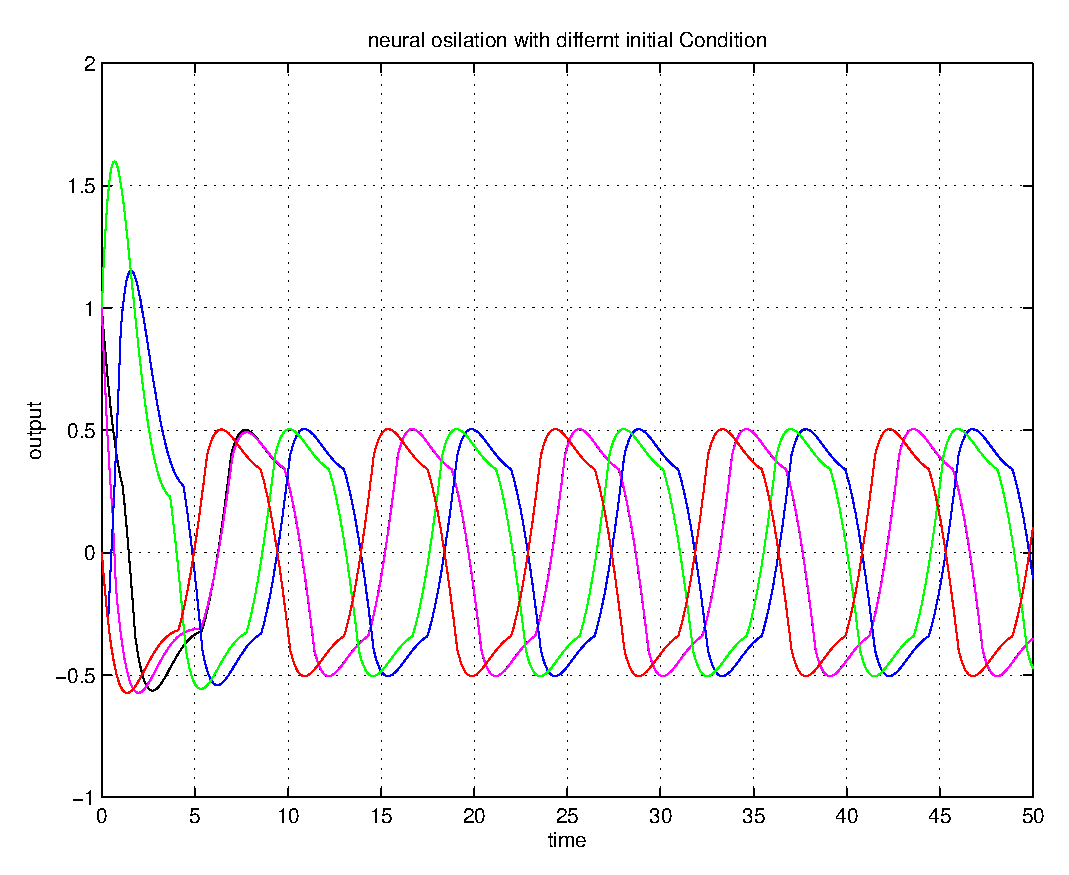
\includegraphics[width=1.5in]{\figurepath/neural_attraction.eps}
\label{fig:time_timeAttraction}
}
\hfill
\subfigure[Phase Portrait]{
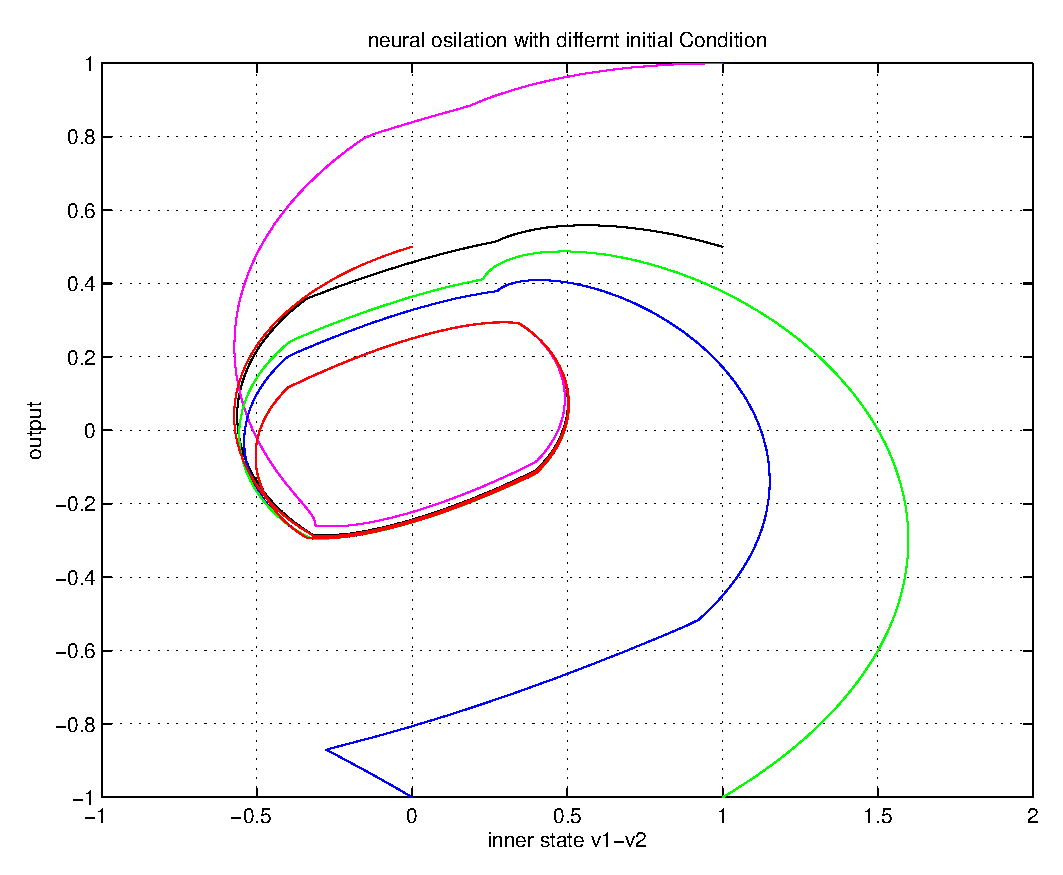
\includegraphics[width=1.5in]{\figurepath/neural_attraction_phase.eps}
\label{fig:phase_attraction}
}
}
\caption{Matsuta Oscilator}
\label{fig:matsuta oscilation}
\end{figure} 

Through this example, we believe neural oscillator is structure stable.
The large area of basin of attraction means the final behavior is totally determined by parameters. 
Initial conditions will have no effects on the final oscillation. 
The converging speed can be seen as quick recovery ability.
When an impulse perturbation happens, it will recover in one period time.

These properties are very valuable in CMS research. 
An intuitive idea is that we couple the neural oscillator with mechanical oscillator of body and environment, thus make the motion structual stable.
